\PassOptionsToPackage{unicode=true}{hyperref} % options for packages loaded elsewhere
\PassOptionsToPackage{hyphens}{url}
%
\documentclass[10pt,a5paper,]{book}
\usepackage{lmodern}
\usepackage{amssymb,amsmath}
\usepackage{ifxetex,ifluatex}
\usepackage{fixltx2e} % provides \textsubscript
\ifnum 0\ifxetex 1\fi\ifluatex 1\fi=0 % if pdftex
  \usepackage[T1]{fontenc}
  \usepackage[utf8]{inputenc}
  \usepackage{textcomp} % provides euro and other symbols
\else % if luatex or xelatex
  \usepackage{unicode-math}
  \defaultfontfeatures{Ligatures=TeX,Scale=MatchLowercase}
\fi
% use upquote if available, for straight quotes in verbatim environments
\IfFileExists{upquote.sty}{\usepackage{upquote}}{}
% use microtype if available
\IfFileExists{microtype.sty}{%
\usepackage[]{microtype}
\UseMicrotypeSet[protrusion]{basicmath} % disable protrusion for tt fonts
}{}
\IfFileExists{parskip.sty}{%
\usepackage{parskip}
}{% else
\setlength{\parindent}{0pt}
\setlength{\parskip}{6pt plus 2pt minus 1pt}
}
\usepackage{hyperref}
\hypersetup{
            pdftitle={QGIS for Transport Research: an introduction},
            pdfauthor={Robin Lovelace},
            pdfborder={0 0 0},
            breaklinks=true}
\urlstyle{same}  % don't use monospace font for urls
\usepackage{color}
\usepackage{fancyvrb}
\newcommand{\VerbBar}{|}
\newcommand{\VERB}{\Verb[commandchars=\\\{\}]}
\DefineVerbatimEnvironment{Highlighting}{Verbatim}{commandchars=\\\{\}}
% Add ',fontsize=\small' for more characters per line
\usepackage{framed}
\definecolor{shadecolor}{RGB}{248,248,248}
\newenvironment{Shaded}{\begin{snugshade}}{\end{snugshade}}
\newcommand{\AlertTok}[1]{\textcolor[rgb]{0.33,0.33,0.33}{#1}}
\newcommand{\AnnotationTok}[1]{\textcolor[rgb]{0.37,0.37,0.37}{\textbf{\textit{#1}}}}
\newcommand{\AttributeTok}[1]{\textcolor[rgb]{0.61,0.61,0.61}{#1}}
\newcommand{\BaseNTok}[1]{\textcolor[rgb]{0.06,0.06,0.06}{#1}}
\newcommand{\BuiltInTok}[1]{#1}
\newcommand{\CharTok}[1]{\textcolor[rgb]{0.5,0.5,0.5}{#1}}
\newcommand{\CommentTok}[1]{\textcolor[rgb]{0.37,0.37,0.37}{\textit{#1}}}
\newcommand{\CommentVarTok}[1]{\textcolor[rgb]{0.37,0.37,0.37}{\textbf{\textit{#1}}}}
\newcommand{\ConstantTok}[1]{\textcolor[rgb]{0,0,0}{#1}}
\newcommand{\ControlFlowTok}[1]{\textcolor[rgb]{0.27,0.27,0.27}{\textbf{#1}}}
\newcommand{\DataTypeTok}[1]{\textcolor[rgb]{0.27,0.27,0.27}{#1}}
\newcommand{\DecValTok}[1]{\textcolor[rgb]{0.06,0.06,0.06}{#1}}
\newcommand{\DocumentationTok}[1]{\textcolor[rgb]{0.37,0.37,0.37}{\textbf{\textit{#1}}}}
\newcommand{\ErrorTok}[1]{\textcolor[rgb]{0.14,0.14,0.14}{\textbf{#1}}}
\newcommand{\ExtensionTok}[1]{#1}
\newcommand{\FloatTok}[1]{\textcolor[rgb]{0.06,0.06,0.06}{#1}}
\newcommand{\FunctionTok}[1]{\textcolor[rgb]{0,0,0}{#1}}
\newcommand{\ImportTok}[1]{#1}
\newcommand{\InformationTok}[1]{\textcolor[rgb]{0.37,0.37,0.37}{\textbf{\textit{#1}}}}
\newcommand{\KeywordTok}[1]{\textcolor[rgb]{0.27,0.27,0.27}{\textbf{#1}}}
\newcommand{\NormalTok}[1]{#1}
\newcommand{\OperatorTok}[1]{\textcolor[rgb]{0.43,0.43,0.43}{\textbf{#1}}}
\newcommand{\OtherTok}[1]{\textcolor[rgb]{0.37,0.37,0.37}{#1}}
\newcommand{\PreprocessorTok}[1]{\textcolor[rgb]{0.37,0.37,0.37}{\textit{#1}}}
\newcommand{\RegionMarkerTok}[1]{#1}
\newcommand{\SpecialCharTok}[1]{\textcolor[rgb]{0,0,0}{#1}}
\newcommand{\SpecialStringTok}[1]{\textcolor[rgb]{0.5,0.5,0.5}{#1}}
\newcommand{\StringTok}[1]{\textcolor[rgb]{0.5,0.5,0.5}{#1}}
\newcommand{\VariableTok}[1]{\textcolor[rgb]{0,0,0}{#1}}
\newcommand{\VerbatimStringTok}[1]{\textcolor[rgb]{0.5,0.5,0.5}{#1}}
\newcommand{\WarningTok}[1]{\textcolor[rgb]{0.37,0.37,0.37}{\textbf{\textit{#1}}}}
\usepackage{longtable,booktabs}
% Fix footnotes in tables (requires footnote package)
\IfFileExists{footnote.sty}{\usepackage{footnote}\makesavenoteenv{longtable}}{}
\usepackage{graphicx,grffile}
\makeatletter
\def\maxwidth{\ifdim\Gin@nat@width>\linewidth\linewidth\else\Gin@nat@width\fi}
\def\maxheight{\ifdim\Gin@nat@height>\textheight\textheight\else\Gin@nat@height\fi}
\makeatother
% Scale images if necessary, so that they will not overflow the page
% margins by default, and it is still possible to overwrite the defaults
% using explicit options in \includegraphics[width, height, ...]{}
\setkeys{Gin}{width=\maxwidth,height=\maxheight,keepaspectratio}
\setlength{\emergencystretch}{3em}  % prevent overfull lines
\providecommand{\tightlist}{%
  \setlength{\itemsep}{0pt}\setlength{\parskip}{0pt}}
\setcounter{secnumdepth}{5}
% Redefines (sub)paragraphs to behave more like sections
\ifx\paragraph\undefined\else
\let\oldparagraph\paragraph
\renewcommand{\paragraph}[1]{\oldparagraph{#1}\mbox{}}
\fi
\ifx\subparagraph\undefined\else
\let\oldsubparagraph\subparagraph
\renewcommand{\subparagraph}[1]{\oldsubparagraph{#1}\mbox{}}
\fi

% set default figure placement to htbp
\makeatletter
\def\fps@figure{htbp}
\makeatother

\usepackage{booktabs}
\usepackage{longtable}
\usepackage[bf,singlelinecheck=off]{caption}

\usepackage{framed,color}
\definecolor{shadecolor}{RGB}{248,248,248}

\renewcommand{\textfraction}{0.05}
\renewcommand{\topfraction}{0.8}
\renewcommand{\bottomfraction}{0.8}
\renewcommand{\floatpagefraction}{0.75}

\renewenvironment{quote}{\begin{VF}}{\end{VF}}
\let\oldhref\href
\renewcommand{\href}[2]{#2\footnote{\url{#1}}}

\makeatletter
\newenvironment{kframe}{%
\medskip{}
\setlength{\fboxsep}{.8em}
 \def\at@end@of@kframe{}%
 \ifinner\ifhmode%
  \def\at@end@of@kframe{\end{minipage}}%
  \begin{minipage}{\columnwidth}%
 \fi\fi%
 \def\FrameCommand##1{\hskip\@totalleftmargin \hskip-\fboxsep
 \colorbox{shadecolor}{##1}\hskip-\fboxsep
     % There is no \\@totalrightmargin, so:
     \hskip-\linewidth \hskip-\@totalleftmargin \hskip\columnwidth}%
 \MakeFramed {\advance\hsize-\width
   \@totalleftmargin\z@ \linewidth\hsize
   \@setminipage}}%
 {\par\unskip\endMakeFramed%
 \at@end@of@kframe}
\makeatother

\renewenvironment{Shaded}{\begin{kframe}}{\end{kframe}}

\usepackage{makeidx}
\makeindex

\urlstyle{tt}

\usepackage{amsthm}
\makeatletter
\def\thm@space@setup{%
  \thm@preskip=8pt plus 2pt minus 4pt
  \thm@postskip=\thm@preskip
}
\makeatother

\frontmatter
\usepackage[]{natbib}
\bibliographystyle{plainnat}

\title{QGIS for Transport Research: an introduction}
\author{Robin Lovelace}
\date{2018-12-16}

\begin{document}
\maketitle

{
\setcounter{tocdepth}{2}
\tableofcontents
}
\hypertarget{preface}{%
\chapter*{Preface}\label{preface}}


This booklet was developed in response to the update from QGIS2 to QGIS3 on centrally managed computer across the University of Leeds'.
That may sound like a minor change, but it meant that previous materials were no longer up-to-date.
Vitally, it meant that some of the instructions simply failed on the latest version of QGIS running on the computers in the `clusters' where many practical sessions in ITS are taught.

Instead of incrementally updating those materials we decided to start from from a blank slate, allowing the inclusion of new datasets and links to excellent on-line content that already exists for QGIS.

The aim is to get you up-to-speed with \emph{the most important concepts and techniques} in QGIS for \emph{Transport Planning}.
We refer to Transport Planning in the broad sense of providing evidence-based guidance to support sustainable transport behaviours.
With air pollution, the obesity crisis, and growing levels of economic inequality in cities worldwide, this inevitably means investment in walking, cycling and public transport.
For this reason the data used in this booklet focusses on these modes.

\hypertarget{pre-requisites}{%
\section*{Pre-requisites}\label{pre-requisites}}


This course assumes that you have access to a working installation of QGIS 3 and an internet connection.
We will explain how to download the data needed for the practicals in Chapter \ref{downloading-and-loading-data}.

\mainmatter

\hypertarget{introduction}{%
\chapter{Introduction}\label{introduction}}

\hypertarget{what-is-gis}{%
\section{What is GIS?}\label{what-is-gis}}

GIS stands for Geographic Information Systems.
The term was first used in the 1960s, and has since become a common way of referring to the analysis of geographic data.

That raises another question: what do we mean by `geographic data'?
The defining feature of geographic data is that it has coordinates that allow the position of records in the dataset to be located on Earth.
There are two main types of geographic data:

\begin{enumerate}
\def\labelenumi{\arabic{enumi}.}
\tightlist
\item
  Vector data, which typically represent points, lines and polygons. An example is a series of points representing a road.
\item
  Raster data, which typically represent a continuously changing surface, such as height.
  An example is a satellite image of a road.
\end{enumerate}

The difference between vector and raster data types is illustrated in the figure below, which shows the same road (Woodhouse Lane in Leeds) represented in vector and raster geographic data forms.

Since graphical user interfaces (GUIs) for GIS became popular in the early 2000s, the word GIS has become almost synonymous with `Dedicated GIS software'.
Examples of dedicated GIS software include the open source GIS software QGIS (we will come onto what QGIS is in a subsequent section) and proprietary software such as ArcMap and TransCAD.
It is also possible, and increasingly popular, to do GIS using a programming language with a command-line interface (CLI) such as Python or R (see \ref{next-steps})

\hypertarget{why-use-gis-for-transport-research}{%
\section{Why use GIS for transport research?}\label{why-use-gis-for-transport-research}}

\hypertarget{what-is-qgis}{%
\section{What is QGIS?}\label{what-is-qgis}}

\hypertarget{alternatives-to-qgis}{%
\section{Alternatives to QGIS}\label{alternatives-to-qgis}}

Now unplug your Internet cable, and start doing some serious work.

More chapters to come in \texttt{02-foo.Rmd}, \texttt{03-bar}.Rmd, \ldots{}

\hypertarget{working-with-qgis}{%
\chapter{Working with QGIS}\label{working-with-qgis}}

Before importing data (covered in Chapter \ref{data}) it is worth getting to know QGIS, in terms of its main components, how to get help, and how it helps you organise your work into projects.

\hypertarget{opening-qgis}{%
\section{Opening QGIS}\label{opening-qgis}}

Probably the quickest way to open QGIS on your computer press `Windows button' on your keyboard and type `qgis' (see Figure \ref{fig:qgis-start}).

\begin{figure}
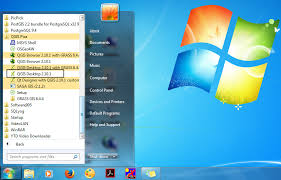
\includegraphics[width=0.5\linewidth]{figures/qgis-start} \caption{Starting QGIS}\label{fig:qgis-start}
\end{figure}

Select `QGIS Desktop' from the list.
If you have multiple versions, choose the latest version.
You should see a new window appear that contains the main features of the QGIS program (see Figure \ref{fig:qgis-window}).
These include the following main components, numbered from 1:5 in the figure and the bullet points below (source: the \href{https://docs.qgis.org/2.18/en/docs/user_manual/}{QGIS Manual}):

\begin{enumerate}
\def\labelenumi{\arabic{enumi}.}
\tightlist
\item
  Menu Bar: like most GUI-based programs you can control key aspects of QGIS and execute key commands, like saving your project and loading new datasets, by clicking Project or Layer. Note: shortcuts to access these menus from the keyboard are \texttt{Alt+J} and \texttt{Alt+L}, respectively.
\item
  Toolbars: these are small icons located towards the top and left hand side of Figure \ref{fig:qgis-window}. In addition to options available from the Menu Bar, these icons provide tools for interacting with the map such as Pan (the hand symbol) and Zoom (the + and - signs).
\item
  Panels: Panels are interactive elements that show information on particular aspects of the project. A view of files in the Browser Panel and the Layers Panel are shown in Figure \ref{fig:qgis-window}.
\item
  Map View: this is where the geographic data is displayed in an interactive map for interactive visualisation.
\item
  Status Bar: this small but important element at the bottom of QGIS shows details about the current status of the Map View, such as the Coordinate Reference System (CRS), in this case EPSG:2964 and scale.
\end{enumerate}

\begin{figure}
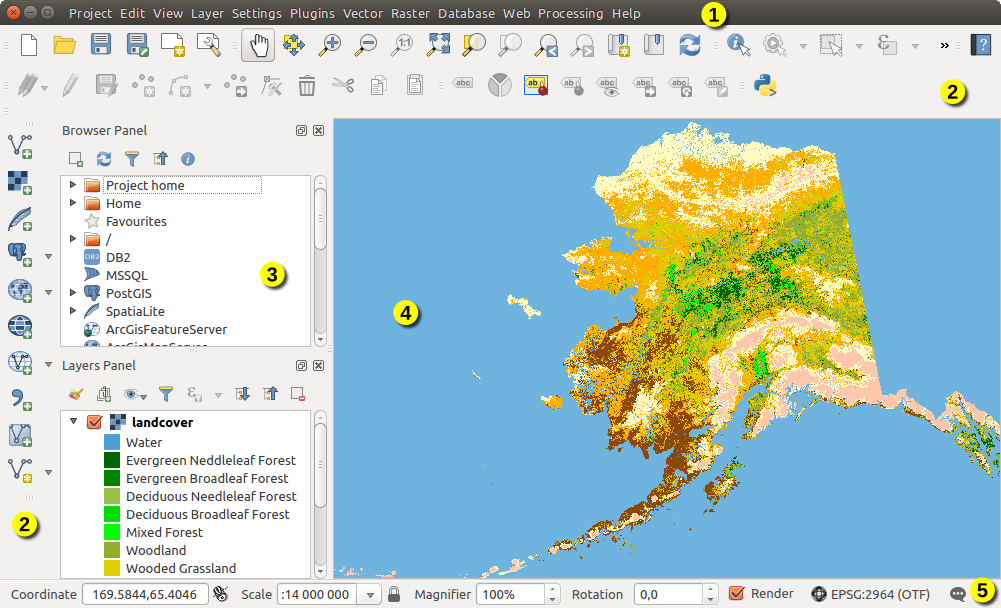
\includegraphics[width=1\linewidth]{figures/startup} \caption{QGIS after opening it for the first time}\label{fig:qgis-window}
\end{figure}

\hypertarget{data}{%
\chapter{Downloading and loading data}\label{data}}

A vital skill for doing using GIS skills to solve real-world problems is finding, downloading and importing data.

Often, the first stage in the data downloading/loading process is to find the data online.
In this case we will access data from the following site, which contains data we prepared earlier for the course: \href{https://github.com/ITSLeeds/SSPA/releases/download/v1.1}{github.com/ITSLeeds/SSPA/releases}.

Look at the file in your explorer\ldots{}

To open a file in QGIS first create a QGIS project.

To load a geographic data file, click on the Data Source Manager button in the top left corner of QGIS (see Figure \ref{fig:data-source-manager}).

\begin{figure}

\includegraphics[width=0.5\linewidth]{figures/open-data-source-manager} \caption{The Data Source Manager icon}\label{fig:data-source-manager}
\end{figure}

\hypertarget{next-steps}{%
\chapter{Next steps}\label{next-steps}}

Examples of programming languages with CLIs include Python and R; some R
code for plotting geographic data is illustrated below.

\begin{Shaded}
\begin{Highlighting}[]
\KeywordTok{library}\NormalTok{(sf)}
\NormalTok{nc =}\StringTok{ }\KeywordTok{read_sf}\NormalTok{(}\KeywordTok{system.file}\NormalTok{(}\StringTok{"shape/nc.shp"}\NormalTok{, }\DataTypeTok{package=}\StringTok{"sf"}\NormalTok{))}
\KeywordTok{plot}\NormalTok{(nc)}
\end{Highlighting}
\end{Shaded}

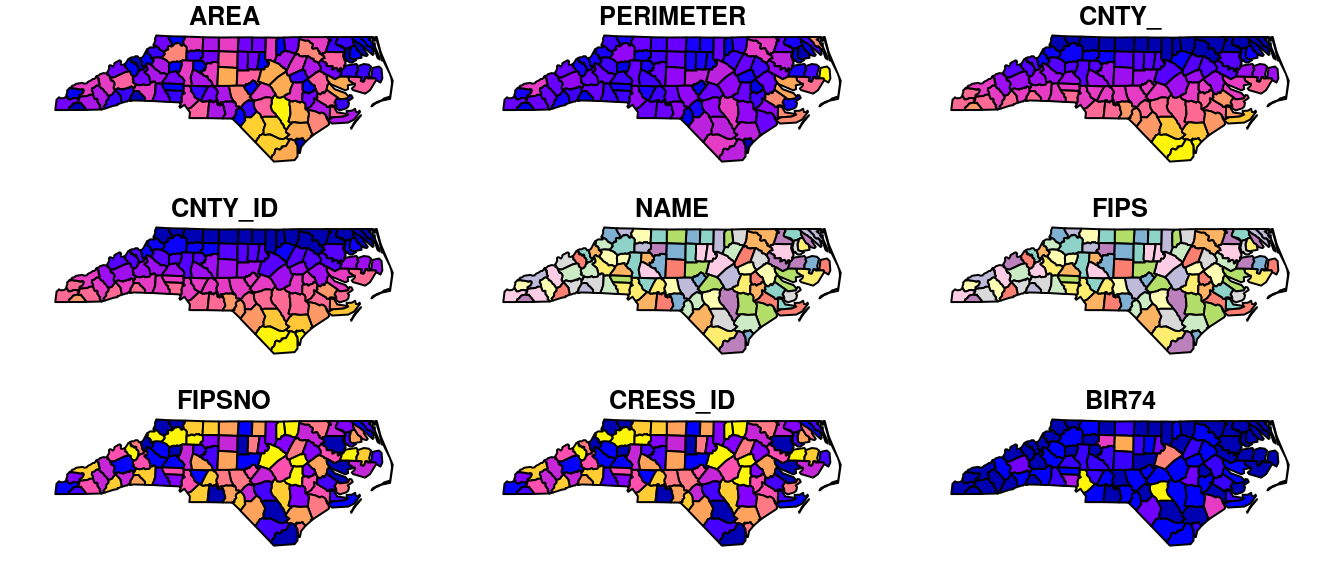
\includegraphics[width=1\linewidth]{bookdown_files/figure-latex/unnamed-chunk-5-1}

\cleardoublepage

\hypertarget{appendix-appendix}{%
\appendix \addcontentsline{toc}{chapter}{\appendixname}}


\hypertarget{more-to-say}{%
\chapter{More to Say}\label{more-to-say}}

Yeah! I have finished my book, but I have more to say about some topics. Let me explain them in this appendix.

To know more about \textbf{bookdown}, see \url{https://bookdown.org}.

\backmatter
\printindex

\end{document}
